\documentclass{article}

\usepackage[english]{babel}

\usepackage[letterpaper,top=2cm,bottom=2cm,left=3cm,right=3cm,marginparwidth=1.75cm]{geometry}

% Useful packages
\usepackage{amsmath}
\usepackage{graphicx}
\usepackage{float}
\usepackage{pgfplots}
\usepackage{caption}
\usepackage{algpseudocode}
\usepackage{algorithm}
\usepackage[colorlinks=true, allcolors=blue]{hyperref}

\algnewcommand\algorithmicforeach{\textbf{for each}}
\algdef{S}[FOR]{ForEach}[1]{\algorithmicforeach\ #1\ \algorithmicdo}

\pgfplotsset{compat=1.18}
\captionsetup{justification=raggedright,singlelinecheck=false}

\newcommand{\smallSpace}{\vspace{0.3cm}}
\newcommand{\mediumSpace}{\vspace{0.5cm}}

\title{Differences between Hill Climbing Algorithm (first improvement, best improvement) and Simulated Annealing Algorithm in finding Global Minimum }
\author{George Buțco}

\begin{document}
\maketitle
\begin{abstract}
In this paper, I compare the time and the minimum value found by a generic Hill Climbing Algorithm (using both first improvement and best improvement) with a simple Simulated Annealing Algorithm.

The comparison will be done using De Jong 1 function\cite{deJong}, Schwefel's function\cite{jamil2013literature}, Rastrigin's function\cite{rastrigin}, Michalewicz's function\cite{back1997handbook} in 5, 10, and 30 dimensions.

I try to prove with examples the following hypotheses:

\begin{enumerate}
  \item Simulated Annealing is faster than Hill Climbing, at least for higher dimensions, but it has a higher error.
  \item Hill Climbing "first improvement" is faster compared to "best improvement", but the minimum value found by "best improvement" is closer to the global minimum.
  \item The only type of function that benefits from using Simulated Annealing over Hill Climbing are wave functions.
\end{enumerate}

\end{abstract}
\section{Introduction}

\textbf{Hill climbing} method is an optimization technique that is able to build a search trajectory in the search space until reaching the local optima. It only accepts the uphill movement which leads it to easily get stuck in local optima.\cite{al2017beta}

\textbf{Simulated annealing} is a well-studied local search meta-heuristic used to
address discrete and, to a lesser extent, continuous optimization problems. The key
feature of simulated annealing is that it provides a mechanism to escape local optima
by allowing hill-climbing moves (i.e., moves which worsen the objective function
value) in hopes of finding a global optimum.\cite{gendreau2010handbook}

As for the \textbf{quantification} of how good an algorithm is, I will choose the best optima found and the time it was found.
\newpage

\section{Implementation}
The function \textit{use-data(time, value)} is the way the main program receives information about the state of the algorithm.

The function \textit{eval(vector)} is a multi-variable function with a single real number as output.

The function \textit{get-current-time()} returns the time passed since the start of the algorithm in seconds as a real number.

The function \textit{neighborhood(vector)} returns all the successors of the vector. 

\subsection{Hill Climbing}

The function \textit{improve(vectors)} returns the first successor better than the current candidate (first improvement) or the best successor among all the vectors (best improvement).


\begin{algorithm}
\caption{Hill Climbing}\label{alg:cap}
\begin{algorithmic}
\Procedure{hc}{\texttt{use-data}, \texttt{eval}}
    \State $t \gets 0$
    \State $best \gets $ \texttt{eval(}random candidate\texttt{)}
     \Repeat
        \State $lower \gets false$
        \State $v_c \gets $ random candidate
        \Repeat
            \State $v_n \gets $ \texttt{improve(neighborhood(}$v_c$\texttt{))}
            \If{\texttt{eval(}$v_n$\texttt{)} is better than \texttt{eval(}$v_c$\texttt{)}} 
                \State $v_c \gets v_n$
            \Else
                \State $lower \gets true$
            \EndIf 
        \Until{$lower$}
        \If{\texttt{eval(}$v_c$\texttt{)} is better than $best$ } 
            \State $best \gets$ \texttt{eval(}$v_c$\texttt{)}
            \State \texttt{use-data( get-current-time(), }$best$\texttt{ )}
        \EndIf 
        
    \Until{$t < MAX$}
\EndProcedure
\end{algorithmic}
\end{algorithm}

\newpage
\subsection{Simulated Annealing}

\begin{algorithm}
\caption{Simulated Annealing}\label{alg:cap}
\begin{algorithmic}
\Procedure{hc}{\texttt{use-data}, \texttt{eval}}
    \State initialize the temperature $T$
    \State $v_c \gets $ random candidate
    \Repeat
        \ForEach {$v_n \in $ \texttt{shuffle( neighborhood(}$v_c$\texttt{) )}}
            \If{\texttt{eval(}$v_n$\texttt{)} is better than \texttt{eval(}$v_c$\texttt{)}} 
                \State $v_c \gets v_n$
                \State \texttt{use-data( get-current-time(), eval(}$v_c$\texttt{) )}
            \Else
                \If{ random[0,1) $ < e^{-\frac{|eval(v_n)-eval(v_c)|}{T}}$} 
                    \State $v_c \gets v_n$
                    \State \texttt{use-data( get-current-time(), eval(}$v_c$\texttt{) )}
                \EndIf 
            \EndIf 
        \EndFor
        \State $T \gets \frac{T}{1+T \cdot \alpha}$
    \Until{$T$ is small enough}
\EndProcedure
\end{algorithmic}
\end{algorithm}

\subsection{Vectors}
A vector with $d$ dimensions is an array of $n \cdot d$ bytes. Every dimension has $n$ bytes that represent an unsigned integer. $v_{max}$ is an unsigned integer where all the bits are $1$.

The conversion from an unsigned integer $x$ to a real number $r$, using $b_l$ as the lower bound and $b_u$ as the upper bound of the function: $$r = \frac{x}{v_{max}}(b_u - b_l)+b_l$$

The precision of a vector($10^{-p}$): $$p = \log_{10}{\left( \frac{ 2^{n \cdot 8}}{b_u- b_l} \right)}$$

\newpage


\section{Comparisons}
\subsection{De Jong 1 Function}

{\large Function Definition:}
\begin{flalign*}
&f(x) = \sum_{i=1}^n x_i^2 \hspace{1cm} -5.12\le x_i \le 5.12&\\
&min(f(x))= 0&\\
&\texttt{Precision used for testing } = 10^{-8.62}&
\end{flalign*}
\smallSpace
\begin{figure}[h!]
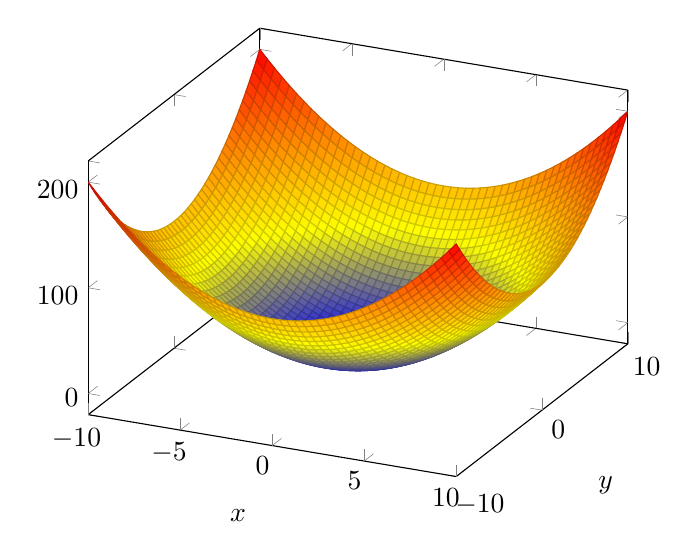
\begin{tikzpicture}
    \begin{axis}[
        xlabel=$x$, ylabel=$y$,
    ]
    \addplot3[surf, domain =-10:10, domain y=-10:10, unbounded coords=jump,
    samples=51]
        { x^2 + y^2 };
  \end{axis}
 \end{tikzpicture}
 
 \caption{Schwefel's Function Graphic}
 \end{figure}
 \mediumSpace
 
 {\large Comparison:}
 \begin{table}[H]
\begin{tabular}{|c|c|c|c|c|c|c|}
\hline
Dimension                      & \multicolumn{6}{c|}{5}                                                            \\ \hline
Algorithm                      & \multicolumn{2}{c|}{HC FI} & \multicolumn{2}{c|}{HC BI} & \multicolumn{2}{c|}{SA} \\ \hline
Time (s) \textbackslash Minima & Time         & Minima      & Time         & Minima      & Time       & Minima     \\ \hline
Best                           & 0.09116     & 0.00000     & 0.00359      & 0.00000     & 0.16880    & 0.00068    \\ \hline
Worst                          & 1.78641     & 0.00000     & 0.00555      & 0.00000     & 1.05987    & 0.00431    \\ \hline
Average                        & 1.02012     & 0.00000     & 0.00427      & 0.00000     & 0.76646    & 0.00213    \\ \hline
\end{tabular}
\end{table}

\begin{table}[H]
\begin{tabular}{|c|c|c|c|c|c|c|}
\hline
Dimension                      & \multicolumn{6}{c|}{10}                                                           \\ \hline
Algorithm                      & \multicolumn{2}{c|}{HC FI} & \multicolumn{2}{c|}{HC BI} & \multicolumn{2}{c|}{SA} \\ \hline
Time (s) \textbackslash Minima & Time         & Minima      & Time         & Minima      & Time       & Minima     \\ \hline
Best                           & 0.16019      & 0.00000     & 0.01376      & 0.00000     & 0.88551    & 0.01190    \\ \hline
Worst                          & 6.11886      & 0.00000     & 0.02351      & 0.00000     & 2.07062    & 0.03498    \\ \hline
Average                        & 3.18844      & 0.00000     & 0.01811      & 0.00000     & 1.63137    & 0.02196    \\ \hline
\end{tabular}
\end{table}

\begin{table}[H]
\begin{tabular}{|c|c|c|c|c|c|c|}
\hline
Dimension                      & \multicolumn{6}{c|}{30}                                                           \\ \hline
Algorithm                      & \multicolumn{2}{c|}{HC FI} & \multicolumn{2}{c|}{HC BI} & \multicolumn{2}{c|}{SA} \\ \hline
Time (s) \textbackslash Minima & Time         & Minima      & Time         & Minima      & Time       & Minima     \\ \hline
Best                           & 0.50992      & 0.00000     & 0.18687      & 0.00000    & 4.48161   & 0.15152   \\ \hline
Worst                          & 61.24491     & 0.00000     & 0.29486      & 0.00000    & 8.16109   & 0.32255   \\ \hline
Average                        & 26.92410     & 0.00000     & 0.21709     & 0.00000    & 5.93557   & 0.22453   \\ \hline
\end{tabular}
\end{table}

\newpage

\subsection{Schwefel's Function}
{\large Function Definition:}
\begin{flalign*}
&f(x)  = \sum_{i=1}^n (-x_i sin(\sqrt{|x_i|})) \hspace{1cm} -500\le x_i \le 500&\\
&min(f(x))= -n\cdot418.9829&\\
&\texttt{Precision used for testing } = 10^{-6.63}&
\end{flalign*}
\smallSpace

\begin{figure}[h!]
  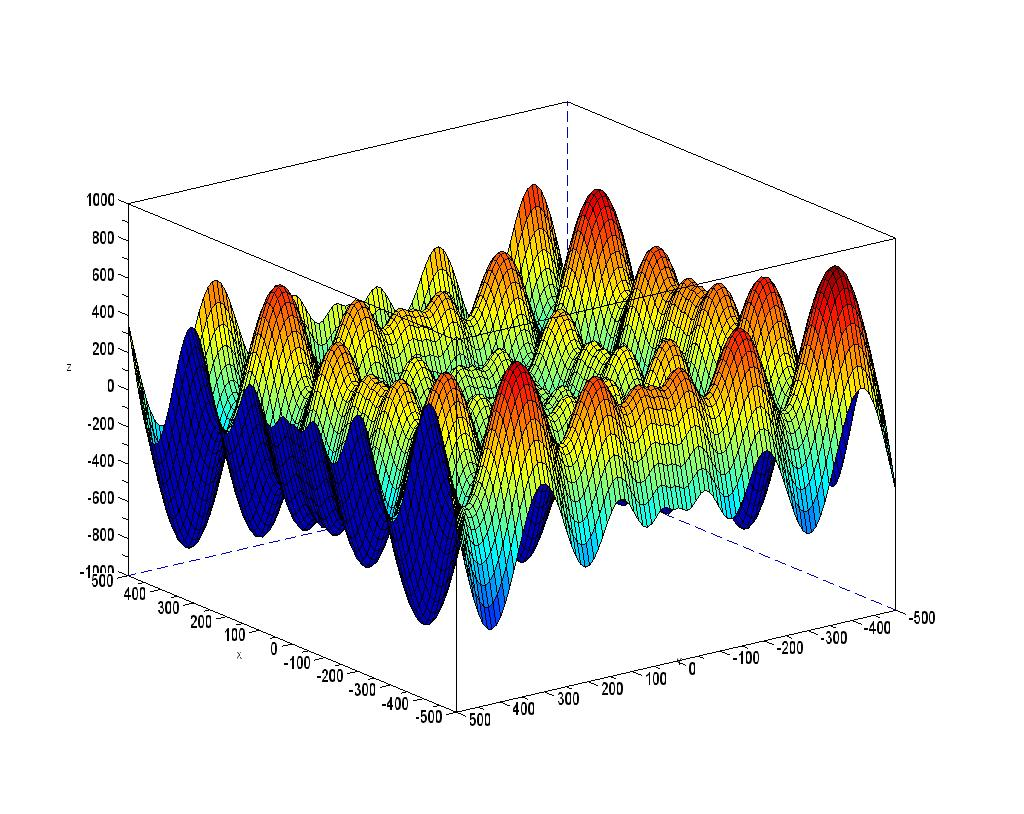
\includegraphics[width=0.6\textwidth]{schwefelsfunction.jpg}
  \caption{Schwefel's Function Graphic\cite{jamesmccaffrey}}
\end{figure}
 
 \mediumSpace
 
 \begin{table}[H]
\begin{tabular}{|c|c|c|c|c|c|c|}
\hline
Dimension                      & \multicolumn{6}{c|}{5}                                                            \\ \hline
Algorithm                      & \multicolumn{2}{c|}{HC FI} & \multicolumn{2}{c|}{HC BI} & \multicolumn{2}{c|}{SA} \\ \hline
Time (s) \textbackslash Minima & Time       & Minima        & Time       & Minima        & Time     & Minima       \\ \hline
Best                           & 0.070228   & -2094.809489  & 0.089141   & -2094.914410  & 0.147038 & -1875.884561 \\ \hline
Worst                          & 3.977570   & -2060.367917  & 4.243352   & -2094.602810  & 1.080576 & -1134.486647 \\ \hline
Average                        & 1.409107   & -2073.465037  & 1.982799   & -2094.820178  & 0.835157 & -1506.567675 \\ \hline
\end{tabular}
\end{table}
 
\begin{table}[H]
\begin{tabular}{|c|c|c|c|c|c|c|}
\hline
Dimension                      & \multicolumn{6}{c|}{10}                                                           \\ \hline
Algorithm                      & \multicolumn{2}{c|}{HC FI} & \multicolumn{2}{c|}{HC BI} & \multicolumn{2}{c|}{SA} \\ \hline
Time (s) \textbackslash Minima & Time       & Minima        & Time       & Minima        & Time     & Minima       \\ \hline
Best                           & 0.800135   & -4070.692393  & 1.450350   & -4189.103207  & 1.341476 & -3597.873265 \\ \hline
Worst                          & 13.416435  & -3750.173074  & 24.727243  & -3998.896753  & 2.581541 & -2492.105525 \\ \hline
Average                        & 6.729373   & -3928.126840  & 10.565069  & -4068.862745  & 1.992218 & -3067.723202 \\ \hline
\end{tabular}
\end{table} 

\begin{table}[H]
\begin{tabular}{|c|c|c|c|c|c|c|}
\hline
Dimension                      & \multicolumn{6}{c|}{30}                                                            \\ \hline
Algorithm                      & \multicolumn{2}{c|}{HC FI} & \multicolumn{2}{c|}{HC BI} & \multicolumn{2}{c|}{SA}  \\ \hline
Time (s) \textbackslash Minima & Time       & Minima        & Time       & Minima        & Time     & Minima        \\ \hline
Best                           & 1.418859   & -11039.503027 & 0.395691   & -11592.659353 & 4.974412 & -10337.482177 \\ \hline
Worst                          & 138.074417 & -10610.823983 & 378.023560 & -11126.868731 & 6.123193 & -8261.315698  \\ \hline
Average                        & 66.605833  & -10847.627730 & 198.344112 & -11378.970798 & 5.743173 & -9422.084350  \\ \hline
\end{tabular}
\end{table}
 
 \newpage
 
 \subsection{Michalewicz's Function}
\begin{flalign*}
&f(x) = - \sum_{i=1}^n sin(x_i) \cdot \left( sin\left( \frac{i\cdot x_i^2}{\pi} \right) \right)^{2 \cdot m} \hspace{1cm} m = 10, 0\le x_i \le \pi&\\
&min(f(x))= -4.687 \hspace{1cm} n=5&\\
&min(f(x))= -9.66 \hspace{1cm} n=10&\\
&\texttt{Precision used for testing } = 10^{-9.13}&
\end{flalign*}

\begin{figure}[h!]
  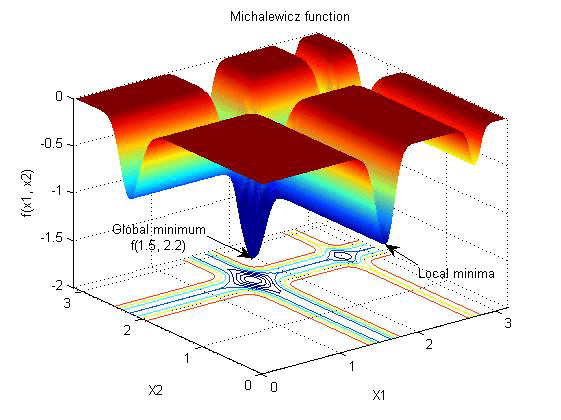
\includegraphics[width=0.6\textwidth]{michalewicz.png}
  \caption{Michalewicz's Function Graphic\cite{researchgate}}
\end{figure}

\begin{table}[H]
\begin{tabular}{|c|c|c|c|c|c|c|}
\hline
Dimension                      & \multicolumn{6}{c|}{5}                                                            \\ \hline
Algorithm                      & \multicolumn{2}{c|}{HC FI} & \multicolumn{2}{c|}{HC BI} & \multicolumn{2}{c|}{SA} \\ \hline
Time (s) \textbackslash Minima & Time        & Minima       & Time        & Minima       & Time       & Minima     \\ \hline
Best                           & 0.032946    & -4.687648    & 0.012815    & -4.687658    & 0.063353   & -4.687046  \\ \hline
Worst                          & 1.858042    & -4.652766    & 7.005613    & -4.682666    & 0.987068   & -4.374004  \\ \hline
Average                        & 1.069647    & -4.681145    & 3.265170    & -4.686512    & 0.606711   & -4.583025  \\ \hline
\end{tabular}
\end{table}


\begin{table}[H]
\begin{tabular}{|c|c|c|c|c|c|c|}
\hline
Dimension                      & \multicolumn{6}{c|}{10}                                                           \\ \hline
Algorithm                      & \multicolumn{2}{c|}{HC FI} & \multicolumn{2}{c|}{HC BI} & \multicolumn{2}{c|}{SA} \\ \hline
Time (s) \textbackslash Minima & Time        & Minima       & Time         & Minima      & Time       & Minima     \\ \hline
Best                           & 0.148167    & -9.468502    & 0.836543     & -9.520684   & 0.301580   & -9.364155  \\ \hline
Worst                          & 8.555991    & -8.873322    & 42.695731    & -9.203955   & 2.129440   & -8.547526  \\ \hline
Average                        & 4.466485    & -9.214113    & 22.206963    & -9.385788   & 1.344480   & -9.089312  \\ \hline
\end{tabular}
\end{table}

\begin{table}[H]
\begin{tabular}{|c|c|c|c|c|c|c|}
\hline
Dimension                      & \multicolumn{6}{c|}{30}                                                           \\ \hline
Algorithm                      & \multicolumn{2}{c|}{HC FI} & \multicolumn{2}{c|}{HC BI} & \multicolumn{2}{c|}{SA} \\ \hline
Time (s) \textbackslash Minima & Time        & Minima       & Time         & Minima      & Time      & Minima      \\ \hline
Best                           & 1.069913    & -26.657838   & 28.435671    & -27.928919  & 3.719086  & -27.709873  \\ \hline
Worst                          & 83.424811   & -25.246337   & 922.223990   & -26.502955  & 6.441927  & -25.271548  \\ \hline
Average                        & 48.286689   & -25.831170   & 435.228857   & -27.076157  & 5.655194  & -26.907374  \\ \hline
\end{tabular}
\end{table}

\newpage

\subsection{Rastrigin's Function}
\begin{flalign*}
&f(x) = 10 \cdot n + \sum_{i=1}^n (x_i^2 - 10 \cdot cos(2 \cdot \pi \cdot x_i)) \hspace{1cm} -5.12\le x_i \le 5.12&\\
&min(f(x))= 0&\\
&\texttt{Precision used for testing } = 10^{-8.62}&
\end{flalign*}

\begin{figure}[h!]
  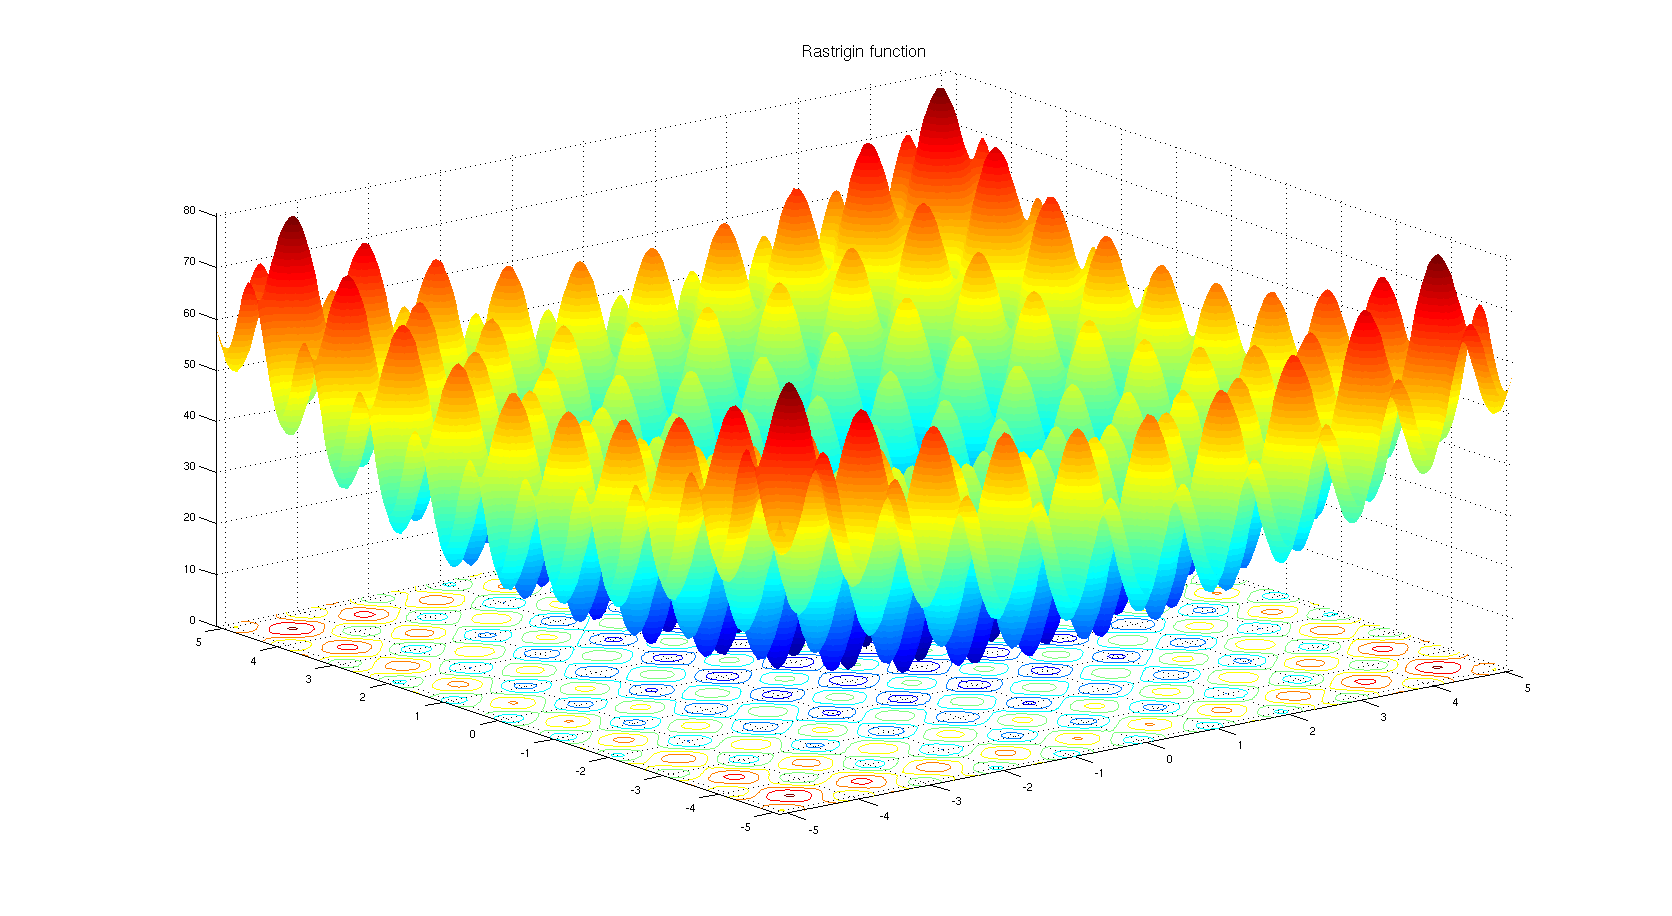
\includegraphics[width=0.6\textwidth]{Rastrigin.png}
  \caption{Rastrigin's Function Graphic\cite{wikiRastrigin}}
\end{figure}

\begin{table}[H]
\begin{tabular}{|c|c|c|c|c|c|c|}
\hline
Dimension                      & \multicolumn{6}{c|}{5}                                                            \\ \hline
Algorithm                      & \multicolumn{2}{c|}{HC FI} & \multicolumn{2}{c|}{HC BI} & \multicolumn{2}{c|}{SA} \\ \hline
Time (s) \textbackslash Minima & Time         & Minima      & Time         & Minima      & Time       & Minima     \\ \hline
Best                           & 0.018603     & 0.000000    & 0.038870     & 0.000000    & 0.162043   & 1.239108   \\ \hline
Worst                          & 2.731234     & 1.994971    & 3.952659     & 1.000000    & 1.043209   & 24.256068  \\ \hline
Average                        & 1.304426     & 1.045690    & 1.692400     & 0.530813    & 0.666320   & 11.050256  \\ \hline
\end{tabular}
\end{table}

\begin{table}[H]
\begin{tabular}{|c|c|c|c|c|c|c|}
\hline
Dimension                      & \multicolumn{6}{c|}{10}                                                           \\ \hline
Algorithm                      & \multicolumn{2}{c|}{HC FI} & \multicolumn{2}{c|}{HC BI} & \multicolumn{2}{c|}{SA} \\ \hline
Time (s) \textbackslash Minima & Time         & Minima      & Time         & Minima      & Time       & Minima     \\ \hline
Best                           & 0.417285     & 2.989766    & 1.338017     & 0.994959    & 1.076592   & 13.679208  \\ \hline
Worst                          & 10.525889    & 8.200483    & 18.573040    & 5.461455    & 2.095559   & 40.873165  \\ \hline
Average                        & 5.183360     & 5.801246    & 11.051008    & 3.856569    & 1.805863   & 26.502426  \\ \hline
\end{tabular}
\end{table}

\begin{table}[H]
\begin{tabular}{|c|c|c|c|c|c|c|}
\hline
Dimension                      & \multicolumn{6}{c|}{30}                                                           \\ \hline
Algorithm                      & \multicolumn{2}{c|}{HC FI} & \multicolumn{2}{c|}{HC BI} & \multicolumn{2}{c|}{SA} \\ \hline
Time (s) \textbackslash Minima & Time         & Minima      & Time         & Minima      & Time      & Minima      \\ \hline
Best                           & 2.773310     & 34.775586   & 3.339413     & 22.394448   & 4.534281  & 52.169252   \\ \hline
Worst                          & 92.607008    & 48.102214   & 301.882618   & 34.277449   & 6.288821  & 115.992046  \\ \hline
Average                        & 42.184061    & 39.989620   & 148.235979   & 28.633780   & 5.699633  & 79.151416   \\ \hline
\end{tabular}
\end{table}

\newpage

\section{Conclusion}
\begin{enumerate}
    \item \textit{"Simulated Annealing is faster than Hill Climbing, at least for higher dimensions, but it has a higher error."}
    
    The average time of Simulated Annealing is better than Hill Climbing for both Wave Functions and paraboloid types of functions.
    The difference in average time between algorithms is higher as the number of dimensions increases.
    
    \textbf{Conclusion:} The Hypothesis is true
    \smallSpace
    \item \textit{"Hill Climbing "first improvement" is faster compared to "best improvement", but the minimum value found by "best improvement" is closer to the global minimum."}
    
    "first improvement" is faster than "best improvement" just when it comes to wave functions. De Jong's Function works better with "best improvement".
    The average minima found by "best improvement" is better for all functions.
    
    \textbf{Conclusion:} The Hypothesis is false.
    
    \textbf{Correction:} "best improvement" is faster for paraboloid types of functions.
    \smallSpace
    \item \textit{"The only type of function that benefits from using Simulated Annealing over Hill Climbing are wave functions."}
    
    For paraboloid types of functions, Hill Climbing works better than Simulated Annealing with a small difference in speed.
    The difference in speed is noticeable for wave functions and as the number of dimensions increases, but the minimum is not as good as using Hill Climbing.
    
    \textbf{Conclusion:} The Hypothesis is false for minima, but true for time.
    
    \smallSpace
\end{enumerate}

\bibliographystyle{ieeetr}
\bibliography{bibliography}

\end{document}